% !TEX root = ./paper.tex

In this section, we evaluate \tcpls using two different types of experiments. First, analyze the raw performance of our \tcpls prototype and the interactions with real middleboxes in a lab with a few servers. We then emulate more complex network scenarios that include failover and multipathing using Mininet~\cite{handigol2012reproducible}.


%Our objective is to evaluate whether our design and implementation are indeed
%fast, flexible and does not conflict with several commercial and open-source
%middleboxes. Moreover, we expect to showcase and compare TCPLS's functionalities
%such as the App-level connection migration, the failover mechanism or the
%bandwidth aggregation capability. We discuss them against the state
%of the art designs, such as mvfst~\cite{mvfast}, quicly~\cite{quicly},
%msquic~\cite{msquic}, MPTCP~\ref{mptcp}, pquic~\cite{pquic},
%quic-go~\cite{quic-go} and MPQUIC~\ref{mpquic}.

%TODO do we also evelatuate security? with a simple proof and discussion?

%To evaluate \tcpls's functionalities, we rely on reproducible network
%experimentations with Mininet~\cite{mininet}. Our objective is to compare the
%behaviour of \tcpls with the state of the art, and to make it easily
%reproducible for future works, as the quic implementations continue to evolve.


\subsection{Raw Performance}
\label{sec:perf}

To evaluate the raw performance (Sec.~\ref{sec:perf}) and middlebox traversal
(Sec.~\ref{sec:middlebox}) of our \tcpls prototype, we use the testbed shown in
Fig.~\ref{fig:perf_testbed}. It contains three servers equipped with Intel Xeon
CPU E5-2630 2.40GHz, 16 Threads, at least 16GB RAM, running Debian with Linux
5.9 and 5.7 kernels. Two of these machines are used as Client and Server, while
the third one is used as a router or a middlebox. Each machine is equipped with
an Intel XL710 2x40GB NIC. With Jumbo frames, a single \tcp connection can
saturate the 40 Gbps path. With a 1500 bytes MTU, a single connection reaches 22
Gbps.

\begin{figure}[!t]
  \begin{center}
    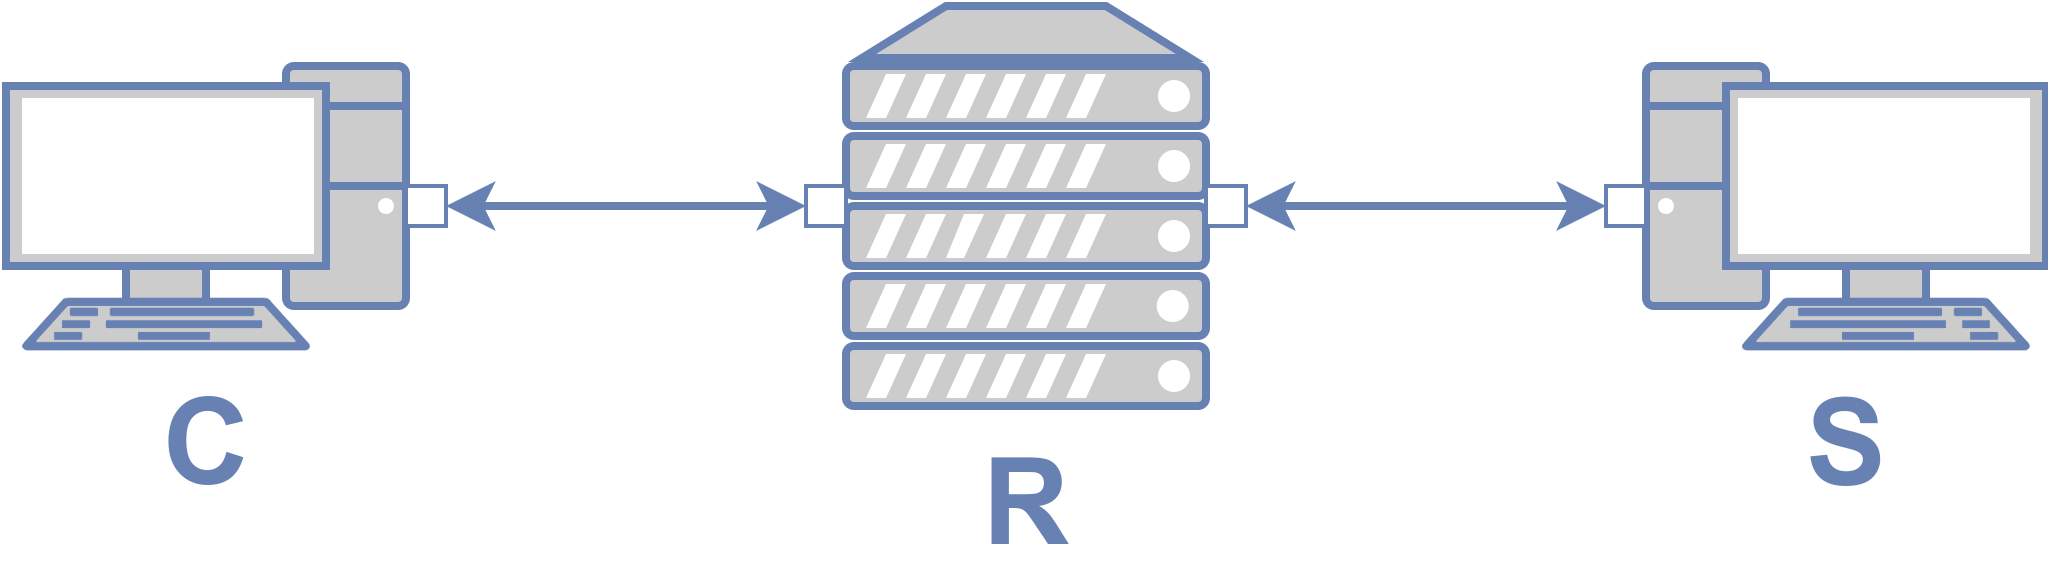
\includegraphics[width=\columnwidth]{figures/testbed.png}
  \end{center}
  \vspace{-0.5cm}
  \caption{Performance Measurements Setups. C = Client. S = Server. R = Router/Middlebox.}
  \label{fig:perf_testbed}
%    \vspace{-0.5cm}
\end{figure}


The first question that we want to answer is whether \tcpls can compete with the traditionnal \tls over \tcp stack. We then compare our \tcpls prototype with different \quic implementations.


\paragraph*{\tcpls}
For all the \tcpls measurements, we used a custom application that performs
large memory-to-memory transfers over a \tcpls session using a single stream.
\tcpls was configured to use the AES128-GCM-SHA256 cipher.
Fig.~\ref{fig:perf} provides the goodput measured in our
testbed. We report both the bandwidth in megabits per second and packets per
second.  Each bar in this figure is the median bandwidth over 10 seconds of stable
throughput. The bottom bar is the highest median goodput that we measured with \tcpls:
12.4 Gbps. This result was obtained with jumbo frames (i.e. 9000 bytes MTU)
and using TCP Segmentation Offload (TSO) on the NICs. TSO is a standard feature
that is enabled by all high-speed NICS. The next bar shows that with TSO and a
standard frame size (1500 bytes MTU), the goodput is still 10.84 Gbps. These
results should be compared with the 22~Gbps that TCP reaches in the same
environment using \texttt{iperf} but without any encryption. We measured that
AES128-GCM-SHA256 peaks at 13.1 Gbps when doing in-memory encrytion/decryption on our
testbed's servers.

%the shows several interesting results. First, while offering similar (and more)
%capabilities than what QUIC is providing today,
%\tcpls is also more than twice faster than the strongest evaluated QUIC
%implementation (quicly) over CPU limited experimentations. We evaluate \tcpls

We then evaluated the impact of adding the \tcpls-level acknowledgements
described in Sec.~\ref{failover} to support failover.
% Thanks to these acknowledgements, \tcpls can support failover.
From a performance viewpoint, they increase the number of control records and
the number of system calls. Our prototype currently sends a \tcpls-ack for every
16 received records. Our measurements indicate that with this functionnality,
\tcpls reaches 9.65 Gbps.


\begin{figure}[!t]
  \begin{center}
    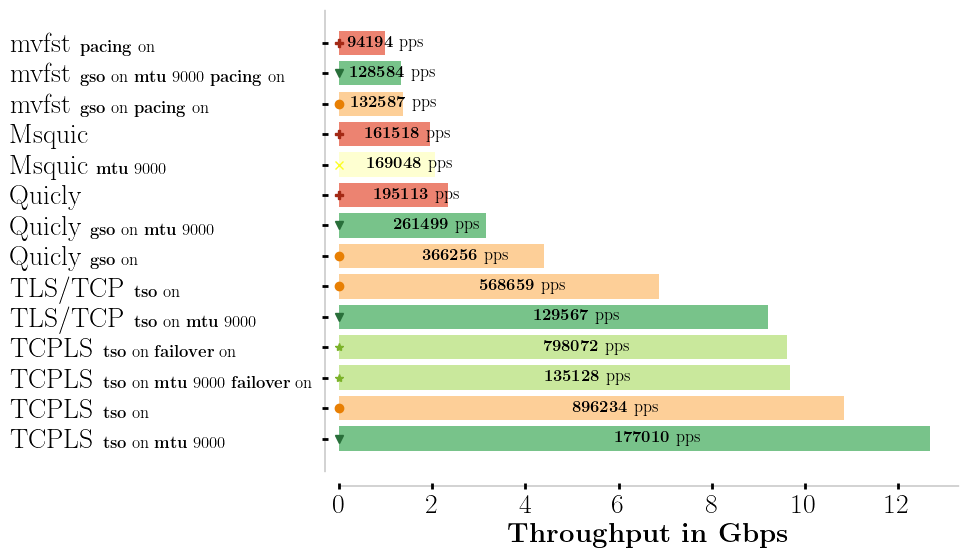
\includegraphics[width=\columnwidth]{figures/perf_analysis.png}
  \end{center}
\vspace{-0.5cm}
  \caption{The \tcpls prototype is faster than \tls over \tcp and different \quic implementations.}
  \label{fig:perf}
\end{figure}


%in four different settings: with a path mtu of 1500 or 9000, and with failover
%enabled or not. The failover functionality is an internal stack feature that
%provides session reliability, which increases the number of syscalls that TCPLS
%makes by exchanging TCPLS-level record acknowledgments. We currently send an
%ac%k for throughput at the price of a slower recovery in case of network
%failure.

\paragraph*{\tcpls vs. \tls/\tcp} We now compare the performance of \tcpls with
the traditional \tls over \tcp stack. To have a fair comparison, we use
\texttt{picotls}'s perf client/server
implementation with the same commit as our initial fork for \tcpls.
Fig.~\ref{fig:perf} shows that \tls/\tcp provides a lower performance than
\tcpls with regular and jumbo frames. This can be explained by the receiving
buffer size provided to \texttt{read()}, which is hardcoded to 16,384 bytes
in \texttt{picotls}'s perf client. This implementation results in fragmentation on the
receiver and prevents it from using the zero-copy code path provided by the
library. \tcpls uses a larger read buffer and benefits from zero-copy. At first,
one may consider this as an unfair comparison, however the devil is in the
details. In \tcpls implementation, the application developers cannot touch
\texttt{read()}'s interface. This implies that an application developer cannot
missuse the relationship between \tls and \tcp by creating fragmented records
and doing unecessary copies to handle those fragments. \tcpls's design and
implementation try to prevent fragmentation by first, having a sufficiently
large read buffer size. Second, \tcpls only starts deciphering a record it has
received the entire record. \tls/\tcp record fragmentation is provided by TLS
libraries as a usability feature that spares the application developers from
taking into account all \tls details, at the cost of lower performance.  With
\tcpls application developers can ignore \tls details without missusing the
interface, which is the reason why this comparison is interesting.\tcpls
constrains the application developer to use the buffer type provided by the API,
but offers zero-copy deciphered records in return.

%\todo{OB: pas sur que la suite est nécessaire} Moreover, but this has not
%yet been implemented, it could be interesting to match the TLS record size to
%the congestion window to deliver faster the data to the application when the
%network is congested.

\paragraph{\tcpls vs. \quic}
Although \quic~\cite{draft-ietf-quic-transport} is a young protocol, there are
already more than a dozen
implementations~\cite{marx2020same,quicimplem,yang2020making} under active
development. We compiled and installed three representative \quic
implementations in our testbed: Facebook's mvfst~\cite{mvfst-github,
  Joras_mvfst} from Facebook, Microsoft's msquic~\cite{msquic-github} Fastly's
quicly~\cite{quicly-github}. They are all developed by large companies that (plan to) use
them in production and include their own benchmarking application to perform
throughput measurements. Furthermore, mvfast and quicly support Generic
Segmentation Offload (GSO), which should improve performance by offloading \udp
segmentation and checksum computation available on our NICs. We use the
implementation's bechmarking application as is, exploiting the optional
arguments provided by their interface to increase the throughput but drawing the
line there. That is, we do not modify the QUIC implementations. Note that, we
tried to match the transport parameters to the same ones used by \tcpls when they did not
adversaly affect QUIC's performance too much. For example, several congestion
algorithms were implemented in the different QUIC implementations, but the a
different value than the suggested default lead to lower performance or unstable
throughput.

The results shown in Fig.~\ref{fig:perf} show that \tcpls compares favorably
with the tested \quic implementations. The fastest \quic implementation is
quicly. Thanks to GSO, it reaches 4.4 Gbps in our testbed with a 1500 bytes
MTU. This result is directly comparable to \tcpls with TSO enabled, which still
performs more than twice faster at 100\% CPU peak with similar configurations
for the receiving buffer size. Suprisingly, quicly's performance decreases with
jumbo frames but is still faster than when GSO is disabled. In our testbed,
msquic could only reach 1,96 Gbps and mvfst was slower despite GSO availability.


%QUIC is young protocol, and all implementations are in active development, with
%different states for their available features and optimizations. For example,
%none of the implementations were able to take advantage of a path mtu larger
%than 1500, and it even degraded the performance in the case of quicly. Two of them
%(quicly and mvfst) have implemented the support for \texttt{gso} leading in the
%case of quicly to more than 4 gb/s of throughput with a udp payload length
%configured to match TCP (1460).


%We perform a throughput evaluation of \tcpls and compare it to several major
%QUIC implementations: mvfst~\cite{} from Facebook, msquic~\cite{} from Microsoft
%and quicly~\cite{} from Fastly. Our choice of QUIC implementations was mainly
%influenced by the availability of a client/server perf tool specifically
%engineered for a throughput evaluation. A second criterion was the advancement
%of the implementation and the quality of the code. We hope to avoid most of the
%bugs negatively impacting their results by selecting the QUIC implementation
%that show advanced features and testings. A third criterion was the development
%language used. \tcpls is written in C, and we prefer to compare it against QUIC
%implementation written in a language compiled by clang or gcc. Mvfst, msquic
%and quicly meet these criteria.


\subsection{Middlebox Interference}
\label{sec:middlebox}

A full evaluation of middlebox interference would require measurements in various operational 
networks that include such devices \cite{honda2011still,raman2020measuring,o2016tls}. This is 
outside the scope of this paper and left for further work.
We tested \tcpls against different opensource and commercial stateful
firewalls and proxy implementations (i.e., pfSense, IPFire, Cisco ASAv,
mitmproxy) and found no unexpected interference. Stateful filtering and stateful
packet inspection policies did not impact connecivity, and transparent TLS proxy
successfully succesfuly triggered \tcpls fallback to \tcp \tls. Still, the security
appliances that block TLS 1.3 or some of its features 
\cite{lee2019matls,Bock_China,raman2020measuring} would also block \tcpls.
%pervasive monitoring allows for configurable TLS extensions blocking
%\cite{rfc7258}. This is handled properly by \tcpls fallback mechanism.


When faced with middleboxes that intercept TLS 1.3
\cite{Bock_China,raman2020measuring}, we need to consider the \tcpls handshake
TLS extensions: \tcpls, \join, \texttt{Connid}, and \texttt{Cookies}. The other
\tcpls messages through the Secure Control Channel are indistinguishable from
classical APPDATA TLS messages (i.e., they look like encrypted application data
for the middlebox). If a clients attempts to open a \tcpls session
through a \tls termination proxy, it sends a \textsc{ClientHello} with the
\tcpls extension.  If the proxy does not support \tcpls, it replies with a
\textsc{ServerHello} message that does not include the \tcpls extension. From
this point, the client implicitely fallback to \tls, and continues with the
handshake.

Certain legacy \tls server implementations are known not to implement the \tls
specification properly and might abort connections when receiving unknown \tls
extensions. Analogous behavior has been observed in overly restrictive stateful
firewalls. To ensure connectivity in the presence of such policies, \tcpls
implements an explicit fallback mechanism. If a client receives a \tcp \rst in
response to the \tcpls-setup \textsc{ClientHello}, or no response, it
tries negotiating a second non-\tcpls \tls connection, either
immediately or after a timeout. Similarly, a \tcpls \join extension might be
blocked on a path. In this case, the subflow attachment is canceled, and
the application is directly notified to be able to react appropriatly (e.g.,
to cancel a migration attempt).

%We tested \tcpls against opensource and commercial stateful firewalls and proxy
%implementations and (i.e., pfSense, IPFire, Cisco ASAv, mitmproxy) and found no
%interferences. Still, certain middlebox security appliances that implement
%pervasive monitoring allows for configurable TLS extensions blocking
%\cite{rfc7258}. This is handled properly by \tcpls fallback mechanism.


\subsection{Bandwidth Aggregation}
\label{sec:bwaggr}
We compare the capability of \tcpls to the state of the art \mptcp. Both
protocols run in the same Mininet topology with two IP paths available, 
\todo{KE: Description of mininet topology comes after this reference}
each 
offering 25 mbps and a latency of 10 ms. The experiment consists to transfering
a file over a single path and then enabling the second one at $5$ seconds. For
\mptcp, the new path is detected after we up the client's second interface. For
\tcpls, managing paths is easier: the application can use the API to add local
or peer-related addresses at any point of the session. In that case, we add
the information at $5$ seconds, connect to the peer and attach a new stream to
this new connection. Our results are displayed in
Fig.~\ref{fig:multipath_aggregation}. Both stacks enable the aggregation of the
goodput to  $\approx$ 50 mbps. There are two major differences displayed by the stacks.
First, upping the interface, adding the routes and detecting the new path in
the case of \mptcp is time consuming. It leads \mptcp to react slower than
\tcpls regarding the availability of the new path. Second, \tcpls's aggregated
goodput seems less stable than \mptcp. This discrepency might explained by the
difference of chunk size manipulated by the reordering algorithm: \mptcp
reorders packets with a payload of $1460$ bytes, while \tcpls in this experiment
reorders records with the maximum payload size of $16384$ bytes. That means
that \tcpls, upon unordered records, would need to reorder and deliver much
larger chunks of data, leading to larger goodput irregularities than \mptcp.
However, \tcpls might  negotiate the record size to smooth out this
irregularity. Setting a record size around $1500$ bytes would make \mptcp and
\tcpls' results lookalike, but would be slightly more CPU costly since we need
to use encryption/decryption code path more often.
Appendix~\ref{appendix:aggr} shows the results of the same experiment but using
a \tls record size of $1500$ bytes instead.

\begin{figure}[!t]
  \begin{center}
    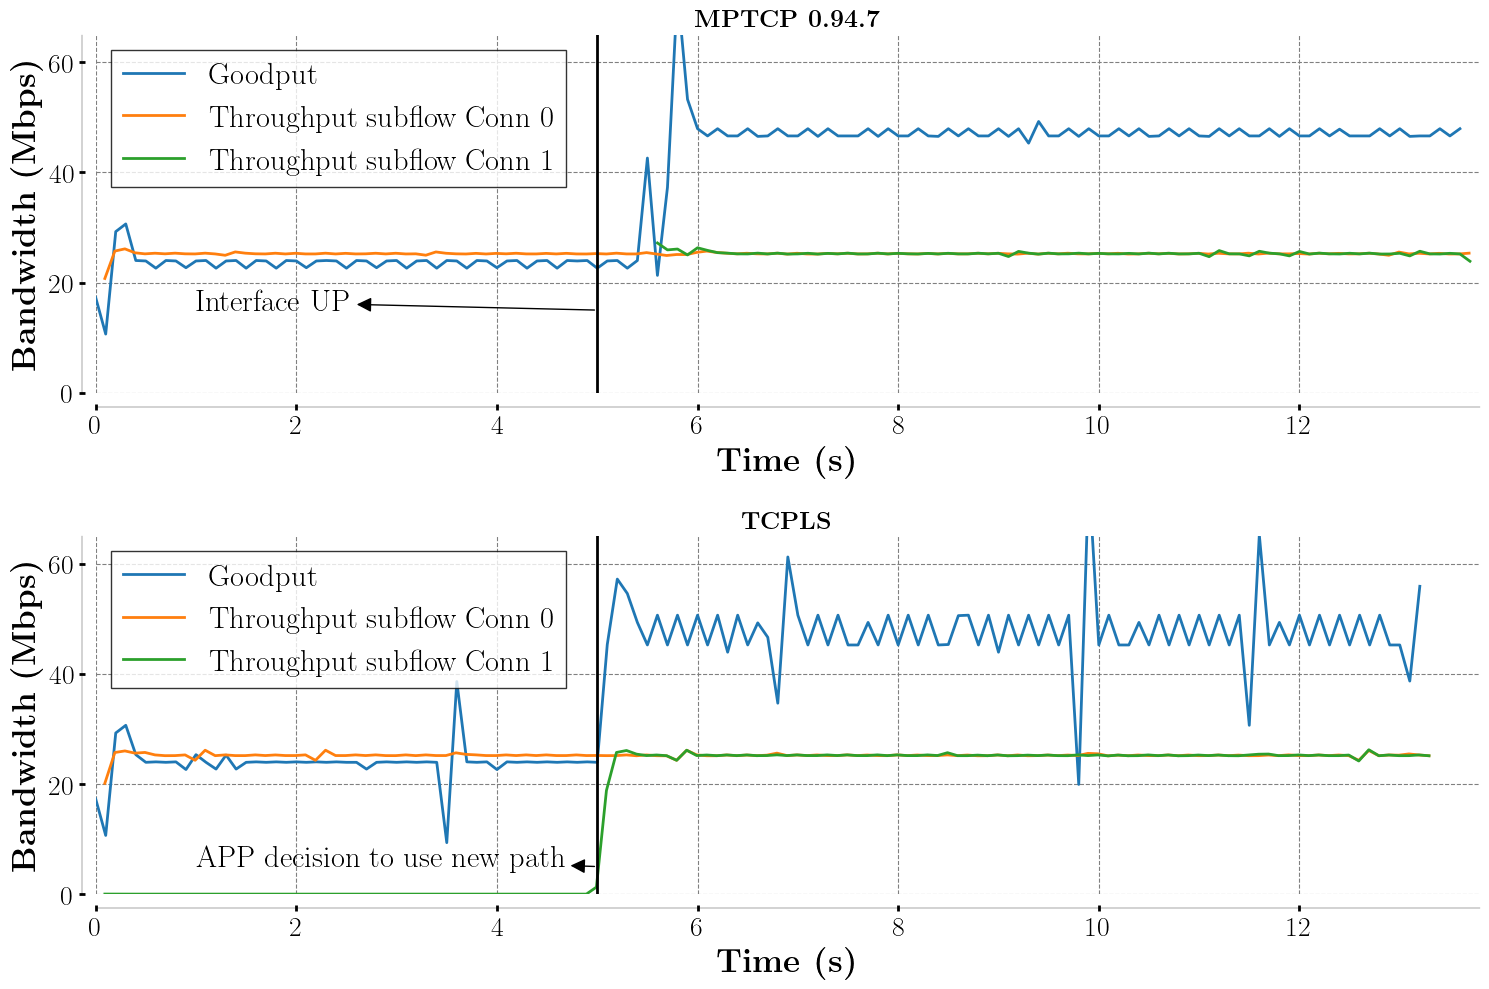
\includegraphics[width=\columnwidth]{figures/aggregate_dual.png}
  \end{center}
\vspace{-0.5cm}
  \caption{Bandwidth aggregation comparison between \mptcp and
    \tcpls with a record payload size of 16384 bytes.}
  \label{fig:multipath_aggregation}
\end{figure}

\subsection{Failover}
\label{sec:eval_failover}

The failover feature is designed to provide reliability to the \tcpls connection
in case of network outage. From middlebox interferences to mobile client loosing
their connection to the access point (LTE or WIFI), network outages may happen
for various reasons. We first discuss and compare the recovery speed
after a network outage, for different types of outage. Fig.~\ref{fig:recovery}
compares the goodput achieved by both \mptcp and \tcpls when they suffer an
outage on their main path and fallback to their secondary path. Both client and
server are configured with two interfaces, with one of them set to the backup
mode in the case of \mptcp (no connections are made to the backup interface
unless an issue is detected on the first path). We consider three types of
outage: a middlebox blackholing all the traffic, the reception of a spurious
$RST$ and the loss of the interface for \mptcp.

\begin{figure}[!t]
  \begin{center}
    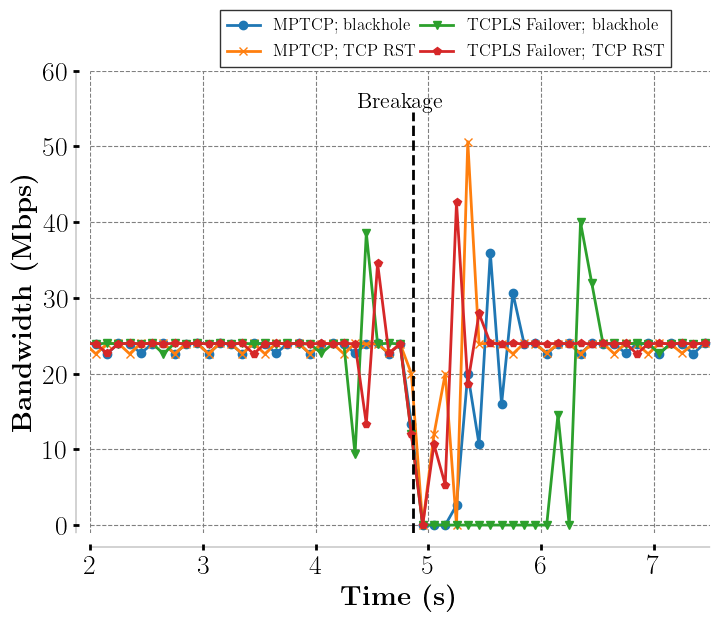
\includegraphics[width=\columnwidth]{figures/breakage_analysis.png}
  \end{center}
\vspace{-0.5cm}
  \caption{Recovery speed analysis.}
  \label{fig:recovery}
\end{figure}

Our results show a range of different behaviours: an explicit issue such as the
reception of a $RST$ makes both \tcpls and \mptcp react fast. A network outage
is more difficult to handle: both stacks configure timers and base their
decision to switch the path on their expiration. In the case of \tcpls, we
configure a timer using the \tcp Option $TCP\_USER\_TIMEOUT$. The scenario is as
follow: when the server sends its data with the failover feature enabled, it
sends a $USER\_TIMEOUT$ to protect the transfer. This option is sent through
the secure control channel to indicate to the client \tcpls's stack that it should
not have to wait more than $X ms$ between successful read of data, with $X$ a
parameter of this option. For this experiment, the $USER\_TIMEOUT$ value is set
to $250ms$. After the timer expiration, \tcpls needs to connect and join the
session through another path, and then replay the unacknowledged records. Once
this steps have succeeded, the transfer can continue. In our experiments, it took
around $\approx 1$ second to recover from the outage.


\begin{figure}[!t]
  \begin{center}
    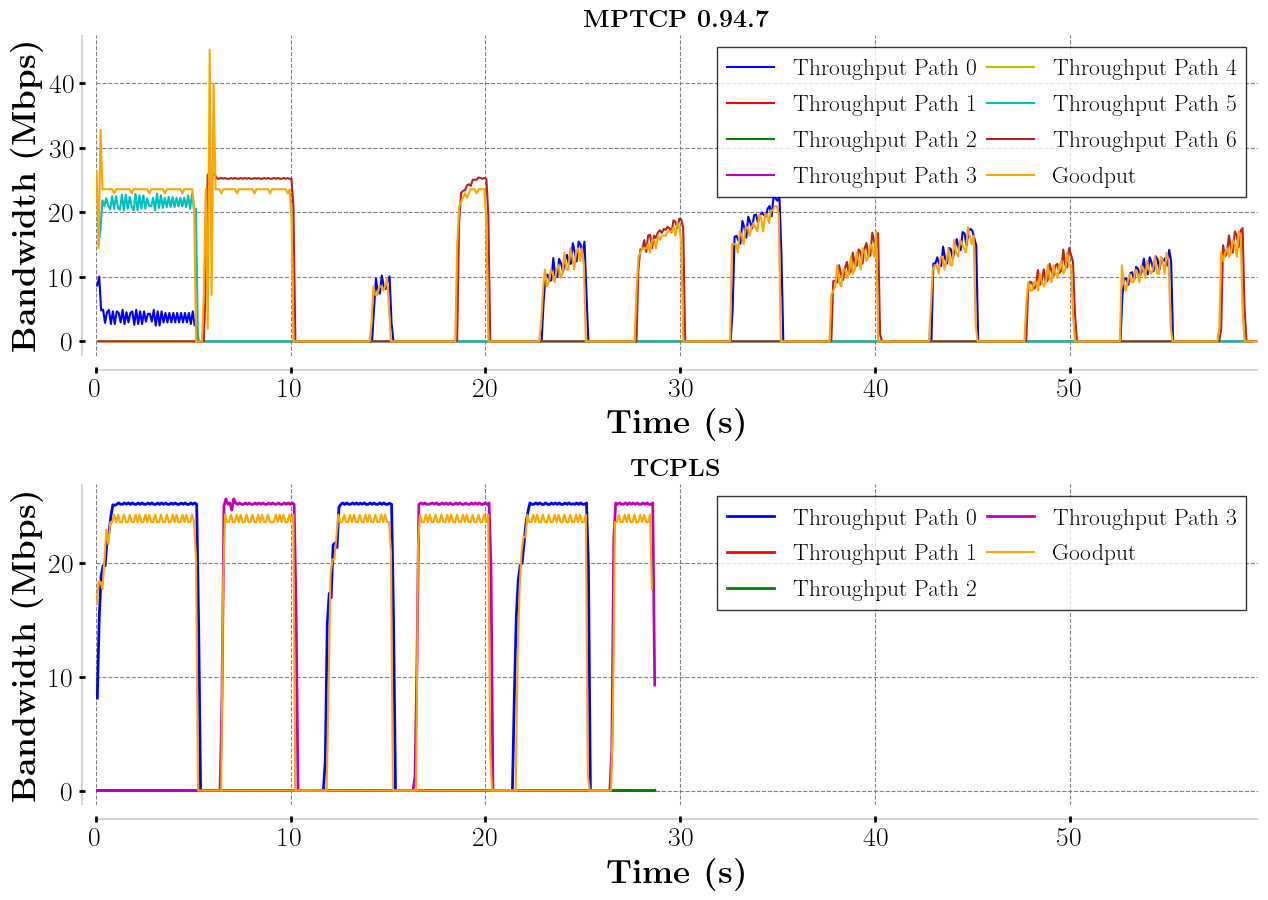
\includegraphics[width=\columnwidth]{figures/tcpls_mptcp.png}
  \end{center}
\vspace{-0.5cm}
  \caption{Connection reliability: influence of the path manager and congestion
    control.}
  \label{fig:failover}
\end{figure}

The second experiment consists into observing how different multipath
implementations behave in case of several failures during a data transfer. We
tested several multipath implementations: \mptcp, PQUIC with the multipath
plugin~\cite{de2019pluginizing} and MPQUIC~\cite{de2017multipath}. The results with PQUIC and MPQUIC were
poor. We dug into their implementations and observed that they were not programmed
to detect network failures and correctly switch the network path, thus we
preferred to ignore those results. However, \mptcp has a longer development
background, is used in production and maintained. Fig.~\ref{fig:failover}
shows how \mptcp and \tcpls performs when 3 paths out of 4 get blackholled every
5 seconds. The path manager has first to find the healthy path and recover the
session over it. We observe that \mptcp performs well on the first
failure. For the next ones, the path manager seems to require several seconds to
recover the right path. Besides, \mptcp remembers that something wrong happened,
and stays inside a congestion avoidance state until the end of the transfer. We
may question this design choice, since many \tcp connections on the Internet have
a shorter lifespan than 10 seconds (i.e., the time after which \mptcp should
re-use a previously used path in this experiment). We also tested multiple
failures based on $RST$, but \mptcp indefinitly stalls after the second $RST$.

\tcpls however, finds the right path and recovers the session as fast as
expected, similarly to the $drop$ and $RST$ outage studied in Figure~\ref{fig:recovery}.
Moreover, since those connections are fresh, the we do not suffer from the same
congestion avoidance than \mptcp.

\subsection{Application-Level Migration}

Given the availability of multiple IP paths, connection migration might be a
powerful tool to improve the application network's reliability. Applications
can take advantage of the \tcpls API to migrate their traffic from one network
path to another. 
Fig.~\ref{fig:conn_migration} shows the result of an Application-level
connection migration demo using the API (i.e., it is left to the application to
decide when to migrate, and we expose a simplistic code flow to perform it). In
this experiment, we use a IPMininet network~\cite{ipmininet,
  jadin2020educational} composed of a client and a server, both
dual-stacks. One path within the network is composed of OSPF routers with IPv4
only, and one path is composed of OSPF6 routers IPv6 only. We configure the
bandwidth on each path to be 30mbps, a round-trip-time of 40ms for the v4 link,
and a round-trip-time of 80ms for the v6 link. Our application downloads
a 60 MB file from a server and migrates twice (i.e., from the v4 to the v6 path
and once again to the v4 path).

Triggering the first connection migration involves chaining 5 API calls: first,
\texttt{tcpls\_handshake()} configured with handshake properties announcing a
\join over the v6 connection id. Then, the creation of a new stream
\texttt{tcpls\_stream\_new()} for the v6 connection id, finally followed by the
attachment of this new stream \texttt{tcpls\_streams\_attach()} and the secure
closing of the v4 \tcp connection using \texttt{tcpls\_stream\_close()}.
Following these events, the server seamlessly switches the path while looping
over \texttt{tcpls\_send} to send the file content. Note that all the events
trigger callbacks on the server side, to let the server react appropriately if
other requirements need to be fulfilled.

Figure~\ref{fig:conn_migration} further shows a peak of goodput at each
migration. During the migration window (marked with vertical black bars
indicating the attachment of the new stream and the closing of the initial
stream), the client is taking advantage of both paths to receive its data: the
first path finishes the flush its data while the second path already started to
send. Once the last record of the first path is sent, \tcpls can reorder the
data and deliver it to the client, which gives this goodput peak matching the
accumulated bandwidth of both paths over the migration time window.

\begin{figure}[!t]
  \begin{center}
    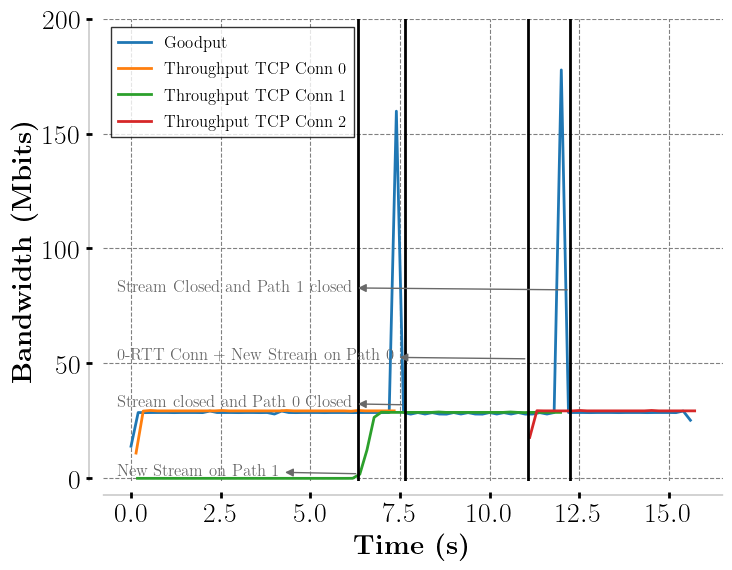
\includegraphics[width=\columnwidth]{figures/migration.png}
  \end{center}
\vspace{-0.5cm}
  \caption{Application-level connection migration during a 60MB file download.
    Showing smooth path handover without goodput loss thanks to a temporary
    bandwidth aggregation.}
  \label{fig:conn_migration}
\end{figure}



\subsection{Dynamically Extending \tcpls}

The \tcpls streams enable new use case. Obviously, a \tcpls application can
create and use different streams to carry data. However, since these streams
are generic, they can also be used by the \tcpls implementation itself to
exchange control information. To demonstrate the versatily of these control
streams, we extended \tcpls to enable a server to push a different congestion
control scheme to a specific client over an existing \tcpls session. Recent
work on restructuring congestion control has proposed a generic architecture
for congestion controllers \cite{narayan2018restructuring}.
During the last years, the Linux kernel developpers have relied on eBPF
to make the Linux TCP/IP stack \cite{brakmo2017tcp,tran2020beyond} easier
to extend. Since Linux kernel version 5.6, an application can inject
a different congestion control scheme entirely implemented using eBPF. A similar
approach was proposed in Pluginizing \quic~\cite{de2019pluginizing}.  We
leverage these new eBPF capabilities to demonstrate the feasibility of injecting
and updating a congestion control scheme during a \tcpls session.

We perform our experiment using Mininet \todo{BD: same remark as above.  Mininet
  or IPMininet} over a 100 Mbps emulated link that has a 60 msec delay.
Fig.~\ref{fig:vegasCubic} shows a client that uses the TCP
Vegas~\cite{10.1145/190314.190317} congestion control scheme to upload a file.
This \tcpls session fully uses the bottleneck link. After some time, another
client starts an upload, but using the CUBIC congestion
controller~\cite{rfc8312}. This results in an unfair distribution of the
bandwidth. The server then sends the eBPF bytecode of the CUBIC congestion
control scheme to the \tcp Vegas client that injects it in its kernel and the
unfairness disappears.  We performed the same experiment for different delay,
varying from 10ms to 100ms.

\begin{figure}[!t]
  \begin{center}
    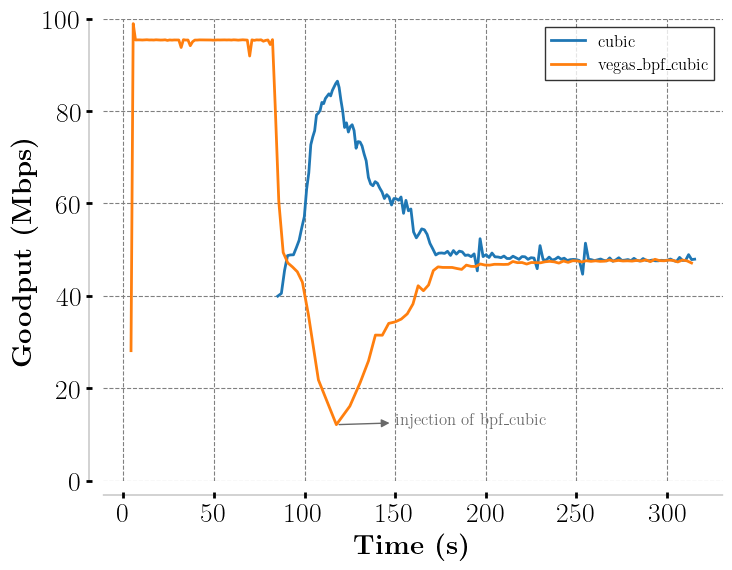
\includegraphics[width=\columnwidth]{pretty_plotify/plots/vegas_cubic.png}
  \end{center}
\vspace{-0.5cm}
  \caption{\tcpls hosts can exchange congestion control schemes and activate them during a \tcpls session.}
  \label{fig:vegasCubic}
\end{figure}
